\documentclass[lettersize,journal]{IEEEtran}
%\usepackage{amsmath,amsfonts}
%\usepackage{algorithmic}
%\usepackage{algorithm}
%\usepackage{array}
%\usepackage[caption=false,font=normalsize,labelfont=sf,textfont=sf]{subfig}
%\usepackage{textcomp}
%\usepackage{stfloats}
\usepackage{url}
\usepackage{verbatim}
\usepackage{graphicx}
\usepackage{cite}
\usepackage{url}
\usepackage{xcolor}
\usepackage{algorithm}
\usepackage{algpseudocode}
\usepackage{amsmath}
\usepackage{booktabs}
\usepackage{threeparttable}
\usepackage{multirow}
\usepackage{graphicx}
\usepackage[numbers]{natbib}
\usepackage{float}
\usepackage{hyperref}


\newcommand{\red}[1]{{\color{black}#1}}
\newcommand{\yellow}[1]{{\color{yellow}#1}}
\newcommand{\ppp}[1]{{\color{purple}#1}}
\newcommand{\blue}[1]{{\color{blue}#1}}
\newcommand{\black}[1]{{\color{black}#1}}

\newcommand{\tsc}[1]{\textsuperscript{#1}}
\hyphenation{op-tical net-works semi-conduc-tor IEEE-Xplore}
% updated with editorial comments 8/9/2021

\begin{document}

\title{}

\author{\IEEEauthorblockN{Lifeng Yan\tsc{1,†}\quad Zhan Zhao\tsc{1,†}\quad Zekun Yin\tsc{1,*}\quad Tong Zhang\tsc{1} \quad Yang Yang\tsc{1} \\ 
\quad Fangjin Zhu\tsc{1} \quad Xiaohui Duan\tsc{1} \quad Bertil Schmidt\tsc{2}\quad Weiguo Liu\tsc{1,*}}\\
\IEEEauthorblockA{
    %\small
    1. School of Software, Shandong University, Jinan, China\\
    \{lifeng.yan, zhaozhan, tong.z, yang.yang\}@mail.sdu.edu.cn\\
    \{zekun.yin, zhufj, sunrise.duan, weiguo.liu\}@sdu.edu.cn\\
    2. Institute for Computer Science, Johannes Gutenberg University, Mainz, Germany\\
    bertil.schmidt@uni-mainz.de\\
    *. Corresponding author \quad †. Co-first authors
}}
%\author{IEEE Publication Technology,~\IEEEmembership{Staff,~IEEE,}
%        % <-this % stops a space
%\thanks{This paper was produced by the IEEE Publication Technology Group. They are in Piscataway, NJ.}% <-this % stops a space
%\thanks{Manuscript received April 19, 2021; revised August 16, 2021.}}

% The paper headers
%\markboth{Journal of \LaTeX\ Class Files,~Vol.~14, No.~8, August~2021}%
%{Shell \MakeLowercase{\textit{et al.}}: A Sample Article Using IEEEtran.cls for IEEE Journals}

%\IEEEpubid{0000--0000/00\$00.00~\copyright~2021 IEEE}
% Remember, if you use this you must call \IEEEpubidadjcol in the second
% column for its text to clear the IEEEpubid mark.

\maketitle

\begin{abstract}

\end{abstract}

\begin{IEEEkeywords}

\end{IEEEkeywords}



\section{Introduction}
The rapid growth of sequencing data continues to increase the computational and storage requirements of genomic data analysis~\cite{amarasinghe2020opportunities,goodwin2016coming,schmidt2017ngs}.After sequence alignment, results are commonly stored in the SAM (Sequence Alignment/Map) or BAM (Binary Alignment/Map) format~\cite{li2009samtools}.These files are subsequently processed by a series of operations, including statistics, filtering, format conversion, sorting, mate information updating, and duplicate marking, before being used by downstream analyses such as variant calling.Many analysis workflows therefore read, reorganize, and rewrite large BAM files multiple times.As sequencing datasets continue to grow, efficient BAM and SAM processing becomes increasingly important for the overall throughput of large-scale genomic analysis.

SAMtools and HTSlib provide the widely used software infrastructure for BAM and SAM processing and support operations such as format conversion, sorting, indexing, and duplicate marking~\cite{danecek2021samtools,bonfield2021htslib}.Several tools have further improved the performance of specific BAM operations.Sambamba uses multi-threaded processing for common alignment-file operations~\cite{tarasov2015sambamba}, while quickBAM provides parallel access to sorted and indexed BAM files~\cite{pitman2023quickbam}.Our previous work, RabbitBAM, focuses on general BAM I/O on multi-core CPU platforms and improves parallel efficiency through pre-parsing, parallel parsing, memory pools, and lock-free queues~\cite{yan2025rabbitbam}.These approaches demonstrate that BAM processing can benefit substantially from architecture-aware optimization.However, their parallel models are mainly designed around conventional CPU threads and do not directly address heterogeneous many-core execution and distributed BAM processing.

The new Sunway architecture provides strong computing capability but also introduces a different execution model.The SW26010-Pro processor consists of multiple Core Groups (CGs), each containing one Management Processing Element (MPE) and 64 Compute Processing Elements (CPEs), while MPI is typically used for communication among processes on different CGs~\cite{zhu2021sunway}.Previous work such as SWQC and SWBWA has shown that bioinformatics applications can achieve high performance on this architecture by moving computation-intensive operations to CPEs and redesigning the original parallel workflow for MPE-CPE execution~\cite{yan2025swqc,yan2026swbwa}.However, BAM processing introduces additional challenges because it combines compressed file I/O, record parsing, format conversion, and application-specific data dependencies.

Efficient BAM processing on Sunway faces three main challenges.First, BAM and SAM libraries naturally expose record-oriented operations, whereas launching and synchronizing CPE tasks for individual records would introduce excessive fine-grained overhead. An efficient design therefore requires both a coarser execution unit and a suitable division of work between the MPE and CPEs. The processing workflow must coordinate MPE-side data preparation and post-processing with CPE computation to reduce synchronization overhead and idle time.Second, distributed BAM processing requires scalable data access and output organization.Multiple MPI ranks should directly process their assigned input regions and generate a valid global output without relying on a single rank to distribute or collect the complete file.Third, BAM applications have very different data dependencies.Simple operations such as statistics and filtering can be performed independently on individual batches, whereas sorting requires global data redistribution, fixmate requires QNAME-based grouping, and duplicate marking requires coordinate-ordered cross-record and cross-rank state.

To address these challenges, we develop SWBAM, a high-performance BAM and SAM processing library and application framework for the Sunway many-core platform.At the library level, SWBAM provides four batch-based MPE-CPE pipelines for BAM reading, BAM writing, SAM reading, and SAM writing.The library separates storage access from computation and supports reusable I/O, batch management, CPE scheduling, and output components.Different processing operators can be attached to these pipelines according to the required operation.SWBAM also optimizes the major CPE kernels for BGZF compression and decompression, BAM parsing, SAM parsing and formatting, and record serialization.At the application level, these common components are reused to implement both streaming operations and distributed BAM algorithms, including statistics, filtering, BAM/SAM conversion, sorting, collation, fixmate, and duplicate marking.The distributed applications further manage global data redistribution, cross-rank communication, and algorithm-specific state.

A key design principle of SWBAM is to provide flexibility at batch boundaries while keeping record-level processing efficient.Pipeline and operator selection is performed at the batch level, whereas performance-critical record operations are statically combined inside CPE kernels.For example, BGZF decompression, BAM parsing, and record-level statistics or filtering can be completed within one CPE launch.This avoids per-record runtime dispatch and unnecessary intermediate processing.Different pipelines can then be connected through MPE-side batch post-processing to construct complete operations such as BAM-to-BAM, BAM-to-SAM, and SAM-to-BAM conversion.In this way, SWBAM improves code reuse while preserving the optimized CPE execution path.

Based on this library, we further develop distributed implementations for more complex BAM operations.
Sorting and collation redistribute records among MPI ranks according to coordinate or QNAME information, respectively.Fixmate handles QNAME groups that may cross batch and rank boundaries.Duplicate marking uses a one-pass coordinate-streaming design with a sliding window, cross-rank boundary handling, and incremental output to control memory usage.These applications are further combined into an end-to-end deduplication workflow consisting of collation, fixmate, coordinate sorting, and duplicate marking.

The main contributions of this work are as follows:
\begin{itemize}
    \item We design SWBAM, a reusable BAM/SAM processing library for the heterogeneous Sunway many-core architecture. SWBAM provides four batch-based MPE-CPE pipelines together with common I/O, double buffering, distributed data access, and output support.
    \item We develop reusable and optimized CPE processing components for BGZF compression and decompression, BAM/SAM parsing and formatting, and record-level operations. SWBAM combines pipelines at batch boundaries and statically fuses record processing inside CPE kernels, reducing fine-grained scheduling and intermediate processing overhead.
    \item We implement distributed BAM applications on top of SWBAM, including sorting, collation, fixmate, and duplicate marking. These applications reuse the common library while introducing application-specific data redistribution, cross-rank state management, and a one-pass coordinate-streaming duplicate-marking algorithm.
    \item We integrate these applications into a complete distributed deduplication workflow and evaluate SWBAM at both the library and application levels on the Sunway platform.
\end{itemize}

\section{Methods}
\subsection{Overview}
% 总体介绍 -> 采取的优化方法
As shown in Fig.~\ref{fig:swbam_overview}, SWBAM consists of two main parts: the SWBAM library and a set of applications built on top of it.The library provides four batch-based processing pipelines for BAM reading, BAM writing, SAM reading, and SAM writing.These pipelines manage data input and output, batch organization, and MPE-CPE execution, providing reusable processing components for different BAM and SAM operations.
For BAM input, compressed BGZF blocks are organized into batches, while SAM input is prepared as text chunks with complete record boundaries.Each batch is processed by the CPEs according to the operation required by the current pipeline.The results are then returned to the MPE for batch-level post-processing and can be further passed to another processing pipeline when required.Based on these common pipelines, SWBAM applications implement complete functions such as format conversion, statistics and filtering, sorting, collating, fixmate, and duplicate marking.

SWBAM applies performance optimizations at both the library and application levels.At the library level, batch-based MPE-CPE processing, double buffering, reusable buffers, and optimized BAM/SAM parsing and BGZF compression and decompression reduce scheduling, synchronization, and data movement overhead.The processing pipelines can also use different operators for different tasks, allowing record-level operations to be performed inside CPE kernels when appropriate.For BAM processing, SWBAM further supports multiple I/O backends and distributed data access across MPI ranks.At the application level, common pipelines and operators are reused to avoid repeated implementation of basic BAM/SAM processing.Applications that require global ordering, record grouping, or cross-record state further employ application-specific distributed algorithms and MPI communication.Together, these designs provide efficient and scalable BAM and SAM processing on the Sunway many-core platform.

\subsection{SWBAM Library Design}
\subsubsection{BAM/SAM input and output}
%io这么设计的原因 -> BAM输入设计及优化 -> SAM输入设计及优化 -> 输出设计
SWBAM provides common input and output interfaces that separate data access from subsequent processing. Different BAM and SAM applications perform different operations, but they share similar requirements for file reading, data partitioning, and result output. Implementing these operations separately for each application would duplicate I/O logic and couple the application algorithm with a specific data access method. SWBAM therefore hides backend-specific I/O operations behind common interfaces and converts the input into batch-oriented data structures required by the processing pipelines. This design allows applications to reuse the same processing implementation when switching between different I/O methods and also provides a common basis for distributed processing across MPI ranks.

For BAM input, SWBAM first scans the compressed data region to identify BGZF block boundaries and builds an ordered block-span index. In MPI execution, the global block index is generated by the root rank and broadcast to all ranks. The indexed BGZF blocks are then divided into contiguous ranges with approximately equal numbers of blocks, and each rank processes only its assigned range. SWBAM supports memory, POSIX, and MPI-IO BAM input backends. The memory backend loads the input file into memory and is mainly used when sufficient memory is available or when evaluating the processing pipeline with limited storage interference. For file-based access, SWBAM scans BGZF headers using an 8-MiB window, reducing the number of small file reads required to identify block boundaries. For contiguous batches, the POSIX backend uses \texttt{preadv} to read multiple BGZF blocks directly into their corresponding block buffers. The MPI-IO backend follows the same block organization and uses an MPI derived datatype to place a contiguous file region directly into multiple BGZF block buffers. These designs reduce small I/O requests and avoid an additional intermediate copy before batch processing.

SAM input follows a similar separation between file access and processing, but uses text ranges instead of BGZF block spans. SWBAM identifies the SAM body after the header and divides it into approximately equal file ranges for distributed execution. Each range boundary is adjusted to a line boundary so that a SAM record is not split between two ranks. The assigned text range is then read through POSIX or MPI-IO and passed to the SAM read pipeline as rank-local input. In-memory input can also be used when the complete input is already available in memory. In this way, BAM and SAM use different data representations while exposing a consistent batch-oriented processing flow to the upper layers.

For output, SWBAM separates the generation of rank-local results from the construction of the final output file. Each rank first stores its generated output body in a rank-local sink. The body can be kept in memory, written to a temporary spool file, or selected automatically according to a configured memory limit. For distributed output, SWBAM collects the body sizes of all ranks and computes their offsets in the final file. The ranks can then write their local bodies directly to the corresponding file regions through MPI-IO, avoiding the need to gather the complete output on a single rank. For BAM output, the global layout contains the BAM header, the ordered rank-local compressed bodies, and a single BGZF EOF block. For SAM output, the text header is followed by the rank-local SAM bodies. This design supports both high-performance in-memory execution and bounded-memory processing of large files.

\subsubsection{Batch-based MPE-CPE pipelines}
%为什么以batch为核心 -> 介绍4条流水线 -> 介绍每一条流水线 -> 介绍双缓冲优化
SWBAM adopts batch-based MPE-CPE pipelines to reduce fine-grained scheduling and synchronization overhead and to improve CPE utilization. Launching CPE tasks at the granularity of individual BAM or SAM records would introduce frequent MPE-CPE coordination and make it difficult to fully utilize the many-core architecture. SWBAM therefore increases the processing granularity from individual records to batches. For BAM processing, multiple BGZF blocks are grouped and processed together, while SAM processing uses batches of text chunks or BAM records according to the direction of conversion. In this way, CPE execution, synchronization, and buffer management are performed at batch boundaries rather than for each individual record.

SWBAM provides four batch-based pipelines for BAM reading, BAM writing, SAM reading, and SAM writing. The BAM read pipeline accepts compressed BGZF batches and invokes a CPE operator that performs decompression and, when required, BAM parsing and application-specific processing. The BAM write pipeline accepts either uncompressed BGZF data or batches of BAM records and performs BGZF compression or record serialization followed by compression. The SAM read pipeline processes text chunks aligned to record boundaries and parses them into BAM records, while the SAM write pipeline formats batches of BAM records into SAM text. Although these pipelines operate on different data representations, they follow a common batch-oriented execution model and provide reusable processing components for upper-level applications.

For each batch, the MPE prepares the input buffers and operator parameters before launching the corresponding CPE kernel. After CPE execution is completed, SWBAM validates the processing status before exposing the results to MPE-side post-processing. The post-processing stage can aggregate batch-level results, submit records to another pipeline, or store application-specific intermediate data. The pipeline owns and reuses its working buffers, while data that need to remain valid across batches are stored in application-owned memory. This design defines clear data ownership and allows different BAM and SAM operations to share the same scheduling framework.

SWBAM further uses reusable alternating buffers to overlap MPE-side work with CPE execution. In the BAM read pipeline, while the CPEs process the current batch, the MPE reads the next compressed batch into another buffer. MPE-side post-processing starts after the current CPE kernel has completed and its results have been validated. In the BAM write pipeline, the MPE can write the previously compressed batch while the CPEs compress the current batch, and the next input batch can also be prepared during CPE execution when required. The SAM write pipeline similarly keeps current and pending output batches, while the SAM read pipeline uses separate CPE stages for text copy/count and record parsing and overlaps MPE-side output handling where possible. These pipeline-specific overlap strategies reduce idle time and reuse allocated buffers across batches without requiring multiple CPE kernels to execute concurrently within the same core group.

\subsubsection{Pipeline composition and operators}
%怎么组合流水线 -> 从核内的operator如何组合 -> 介绍两个SDK示例 -> 一些优化
SWBAM supports flexible BAM and SAM processing by composing pipelines at batch boundaries and integrating record-level operations within CPE kernels. The four processing pipelines provide the common mechanisms for I/O, buffer management, CPE scheduling, and synchronization, while operators define the processing performed on each batch. For the BAM read pipeline, an operator prepares the batch parameters, selects the corresponding CPE kernel, validates the processing results, and performs batch-level post-processing on the MPE. These operator interfaces are invoked once for each batch rather than for each BAM record, avoiding fine-grained dispatch overhead in record processing.

Within a CPE kernel, SWBAM further combines common BAM processing steps with different record-level operations. The BAM read implementation reuses the same decompression and record traversal framework for operations such as record counting, flag statistics, basic statistics, filtering, and passthrough processing. The selected record operation is determined when the CPE kernel is built, so decompression, parsing, and the required record processing can be completed within a single CPE launch. This avoids per-record virtual calls and reduces intermediate processing between separate kernels. The operator can then return batch-level records, statistics, or application-specific metadata to the MPE for subsequent processing.

Different pipelines can be further connected through MPE-side batch post-processing to construct complete BAM and SAM operations. For example, record counting only uses the BAM read pipeline with a counting operator and aggregates the batch results on the MPE. BAM-to-BAM processing connects a BAM read operator with the BAM write pipeline. The read operator performs decompression, parsing, and optional filtering, after which the MPE builds record packing plans and submits them to the write pipeline for serialization and BGZF compression. Similarly, BAM-to-SAM processing connects the BAM read pipeline with the SAM write pipeline, while SAM-to-BAM processing connects the SAM read pipeline with the BAM write pipeline. In these cases, records are exchanged between pipelines at batch boundaries rather than through a new record-level dispatch layer.

SWBAM also defines clear ownership rules for data shared between pipelines. Pipeline buffers are reused across batches and are valid only during their corresponding processing stage. Records or intermediate data that must remain valid across batch boundaries are explicitly copied to application-owned memory. This design allows the same pipelines and operators to be reused by different applications while keeping the record-processing hot path on CPEs. As a result, SWBAM improves code reuse without introducing additional per-record abstraction overhead.

\subsubsection{CPE kernel optimizations}
%压缩解压侧的优化 -> 输入侧的融合优化 -> 输出侧的融合优化 -> sam的相关从核优化 
SWBAM further optimizes the major BAM and SAM processing kernels executed on CPEs to reduce computation, memory allocation, and intermediate data movement. BGZF compression and decompression are repeatedly invoked during continuous BAM processing, and repeatedly creating the corresponding codec objects introduces unnecessary overhead. SWBAM therefore maintains reusable libdeflate compressor and decompressor objects for individual CPEs. A decompressor is created when first used and is then reused by the same CPE across subsequent batches. Compressors are similarly cached according to the compression level and recreated only when the required level changes. For the performance-oriented level-1 compression path, SWBAM further adjusts the match-search strategy to reduce the work spent on compression while retaining valid BGZF output.

BAM parsing is also performed directly on CPEs and is integrated with record-level processing. After a BGZF block is decompressed, SWBAM traverses the BAM records in the decoded block using a common parser. Frequently used record operations, including counting, flag statistics, basic statistics, filtering, and passthrough processing, reuse the same traversal framework. The selected operation is resolved when the CPE kernel is built and is executed directly during record traversal. Thus, BGZF decompression, BAM parsing, and the required record operation can be completed within one CPE launch without per-record runtime dispatch. SWBAM also reuses preallocated record buffers and scratch spaces across records and batches, reducing repeated memory allocation during parsing.

SWBAM applies a similar fusion strategy to BAM output. When the input is already organized as uncompressed BGZF blocks, the CPEs directly compress these blocks. When the input consists of BAM records, SWBAM first serializes the records into BGZF-ready blocks and then performs compression within the same CPE execution. This avoids constructing another complete BAM representation on the MPE between serialization and compression. The output buffers and temporary scratch spaces are reused across batches, further reducing memory management overhead.

The SAM pipelines are also implemented with CPE kernels for the major processing stages. SAM reading first partitions text into record-aligned chunks and uses CPE kernels for text copy/count and record parsing. SAM writing formats batches of BAM records into SAM text on CPEs. Together with the batch-based execution model described above, these kernel-level optimizations move the major parsing, formatting, compression, and decompression work to CPEs while reducing repeated allocation and intermediate processing on the MPE.

\subsection{Applications Built on SWBAM}
\subsubsection{Streaming BAM processing}
%什么是流式处理 -> 统计类操作 -> bam2bam -> bam2sam和sam2bam -> 简单总结
SWBAM implements several streaming BAM and SAM operations that process the input in a single pass without global record reordering. These operations include flag statistics, basic statistics, BAM filtering and rewriting, and format conversion between BAM and SAM. Since the processing of one batch does not depend on distant records, each MPI rank can independently process its assigned input range using the common SWBAM pipelines. Only small final results, such as statistics or output layout information, need to be exchanged among MPI ranks.

For statistical operations, SWBAM uses the BAM read pipeline with application-specific CPE operators. The flagstat and basic-statistics operators combine BGZF decompression, BAM parsing, and record-level statistics within the CPE kernel. Each batch produces rank-local counters, which are accumulated on the MPE after CPE processing. After all local batches are processed, the rank-local results are combined through MPI reduction to generate the final statistics. This design avoids materializing an additional BAM stream and keeps the main record processing on CPEs.

BAM filtering and rewriting are implemented by connecting the BAM read and BAM write pipelines. The read-side transform operator performs decompression, parsing, and optional record filtering. The retained records are then organized into record packing plans on the MPE and submitted to the BAM write pipeline, where record serialization and BGZF compression are performed on CPEs. For records that are removed by the filter, no output record is generated. The same pipeline can also operate in passthrough mode when no filtering is required. Each MPI rank produces its own ordered output body, which is later placed at the corresponding position in the final BAM file.

Format conversion is implemented by composing the corresponding read and write pipelines. For BAM-to-SAM conversion, the BAM read pipeline decompresses and parses the input records using the passthrough operator, and the parsed records are passed in batches to the SAM write pipeline for parallel formatting on CPEs. For SAM-to-BAM conversion, the SAM read pipeline first identifies complete SAM records and parses them into BAM records, after which the BAM write pipeline serializes and compresses the records into BGZF blocks. The intermediate records are only kept for the current batch and are released or reused after the downstream pipeline completes its processing. This batch-level composition preserves record order while avoiding an additional record-level dispatch layer between the two pipelines.

Compared with the distributed algorithms described below, these streaming operations require little cross-rank communication. Most computation and data movement are performed locally within each rank, while MPI is mainly used for final statistics aggregation and distributed output organization. Therefore, they directly benefit from the batch-based MPE-CPE pipelines and provide representative applications for evaluating the basic processing efficiency of SWBAM.

\subsubsection{Distributed BAM processing}
%先总体介绍 -> sort/collate -> fixmate -> markdup
SWBAM further implements distributed BAM operations that require global data reorganization or cross-record state. Unlike streaming operations, these applications cannot process each MPI rank completely independently because records belonging to the same global order, QNAME group, or duplicate group may be distributed across different ranks. SWBAM therefore reuses the common BAM read and write pipelines for local data processing, while the application layer manages algorithm-specific metadata, MPI communication, and global state. This design keeps BGZF I/O and CPE processing reusable while allowing each application to adopt a distributed algorithm suited to its data dependency.

\paragraph{Sorting and collation}
Sorting and collation both require global redistribution of BAM records, but use different partitioning keys. For coordinate sorting, SWBAM first uses CPEs to extract the coordinate key and raw BAM data from each record. Each rank sorts its local metadata and selects samples from the ordered records. The samples are collected to determine global splitters, which divide the coordinate space among MPI ranks. Local records are then partitioned according to these splitters and exchanged with their destination ranks. Since the records sent from each source rank are already ordered, the receiving rank performs a k-way merge of the received segments instead of sorting all received records again. The final raw records are directly packed into BGZF payloads and compressed through the common BAM write pipeline. When the data exceed the configured memory limit, SWBAM generates sorted runs and performs bounded data exchange and streaming multi-way merging, allowing the same distributed sorting scheme to operate in external-memory mode.

Collation follows a similar distributed organization but groups records according to QNAME instead of genomic coordinates. During BAM reading, CPEs extract the QNAME hash, QNAME-related metadata, and raw record data. Records are assigned to bins, and each bin is mapped to an owner rank so that records with the same QNAME are processed by the same rank. After local ordering, self-owned records are retained locally, while records owned by other ranks are exchanged in bounded chunks. The received segments are then merged according to their QNAME order, keeping records from the same QNAME together and preserving the required ordering within a group. Similar to sorting, SWBAM provides both in-memory and external-memory implementations. The external mode stores intermediate runs under the configured memory limit and uses streaming multi-way merging before the results are passed to the BAM write pipeline.

\paragraph{Fixmate}
Fixmate requires records with the same QNAME to be processed as a group and therefore introduces state across batch and rank boundaries. SWBAM reads the name-collated input through the common BAM read pipeline and groups consecutive records with the same QNAME on the MPE. Complete groups are processed immediately, while incomplete groups at batch boundaries are retained until the following batch is available. A QNAME group may also cross an MPI rank boundary. SWBAM identifies these boundary groups and transfers their fragments to a selected owner rank before mate information is updated. For each complete group, a CPE planning kernel determines the required mate-field and tag updates and the output size. The MPE then computes output offsets, and a second CPE kernel rewrites the records in parallel. The current implementation updates mate coordinates, flags, template length, and the \texttt{MQ}, \texttt{MC}, and \texttt{ms} tags required by the supported fixmate mode. The rewritten records are finally serialized and compressed through the common BAM write pipeline.

\paragraph{Duplicate marking}
Duplicate marking is implemented for coordinate-ordered BAM data and requires both cross-record comparison and cross-rank coordination.SWBAM first uses the BAM read pipeline to decode and parse input batches, while application-specific CPE processing extracts only the information required for duplicate detection.Candidates are assigned to owner ranks according to their coordinate ranges, so that most candidates remain on the local rank and only candidates belonging to another coordinate range need to be exchanged.Each owner rank maintains separate states for paired and single-read candidates and compares records with the same duplicate key to determine the record to retain.

%markdup伪代码
\begin{algorithm}[!t]
\caption{Distributed duplicate marking on rank $r$}
\label{alg:distributed_markdup}
\small
\hspace*{\algorithmicindent}\textbf{Input:} Coordinate-sorted BAM blocks assigned to rank $r$;
maximum read length $L$\\
\hspace*{\algorithmicindent}\textbf{Output:} Rank-local duplicate-marked BGZF body
\begin{algorithmic}[1]
%\State $H_r \gets \Call{BuildBoundaryPlan}{L}$
%\Comment{Probe rank edges; pre-resolve boundary candidates if covered}
\State $P_r \gets \Call{ProbeHeadAndTailBlocks}{r}$
\State $G \gets \Call{AllGatherRankStartCoordinates}{ }$
\State $covered \gets \Call{HaloCoveredOnAllRanks}{P_r,G,L}$
\If{$covered$}
    \State $E_r \gets \Call{SelectBoundaryCandidates}{P_r,G,L}$
    \State $H_r \gets \Call{ExchangeResolveAndReturnDecisions}{E_r,G}$
\Else
    \State $H_r \gets \mathrm{disabled}$
    \Comment{Retain boundary candidates in the conservative window}
\EndIf

\State Initialize candidate window $W_r$, pending block queue $Q_r$,
       and body writer $O_r$
\State $T \gets \Call{AllReduceMax}{\text{number of local batches}}$

\For{$t=1,\ldots,T$}
    \State $(B,C_r,p_r) \gets \Call{DecodeAndExtractBatchOrEmpty}{t}$
    \Comment{CPE decoding, parsing, and candidate extraction}
    \State Append decoded blocks of $B$ to $Q_r$ with provisional
           KEEP states
    \State Apply pre-resolved decisions from $H_r$ to $Q_r$
    \State Remove pre-resolved boundary candidates from $C_r$

    \State $(C_r^{\mathrm{local}},C_r^{\mathrm{remote}})
           \gets \Call{PartitionByCoordinateOwner}{C_r}$
    \State Mark source records of $C_r^{\mathrm{remote}}$ as pending
    \State $C_r^{\mathrm{owner}} \gets C_r^{\mathrm{local}}
           \cup \Call{ExchangeCandidates}{C_r^{\mathrm{remote}}}$
    \State \Call{AdvanceOptimisticWindow}
           {$W_r,C_r^{\mathrm{owner}},p_r,L,Q_r,D_r^{\mathrm{remote}}$}
    \Comment{Apply local KEEP/DUP or pending actions immediately}
    \State $D_r^{\mathrm{received}}
           \gets \Call{RouteDecisionsToSource}{D_r^{\mathrm{remote}}}$
    \State Apply $D_r^{\mathrm{received}}$ to pending records in $Q_r$
    \State \Call{WriteReadyPrefix}{$Q_r,O_r$}
\EndFor

\State Validate coordinate order across ranks
\State Finalize remaining candidates in $W_r$ as KEEP
\State Route remaining remote decisions to source ranks
\State Apply received decisions to $Q_r$
\State \Call{WriteReadyPrefix}{$Q_r,O_r$} until $Q_r$ is empty
\State Finish compression and $O_r$

\Statex
\Procedure{WriteReadyPrefix}{$Q_r,O_r$}
    \While{$Q_r \neq \emptyset$ \textbf{and}
           the front block has no unresolved records}
        \State Remove the front decoded block $P$ from $Q_r$
        \State Set duplicate flags in $P$ according to finalized states
        \State Compress and append $P$ to $O_r$
        \State Release $P$ after output completion
    \EndWhile
\EndProcedure
\end{algorithmic}
\end{algorithm}

To bound memory usage, SWBAM performs duplicate marking in a one-pass coordinate-streaming manner.Candidates are processed in coordinate order using a sliding window, and candidates that can no longer interact with future records are retired from the active state.Records close to MPI rank boundaries require additional handling because their duplicate partners may reside on neighboring ranks.SWBAM therefore builds a boundary halo around rank partitions and exchanges the required candidate information before final decisions are made.Decoded blocks whose duplicate decisions are not yet complete are temporarily retained in a bounded pending queue.Once all local and remote decisions for a block are available, SWBAM updates the duplicate flags and incrementally submits the ready block to the common BAM write pipeline.The common library manages batch scheduling and output, while the application maintains the sliding window, MPI decisions, boundary state, and pending records.

\subsubsection{Deduplication workflow}
%这四步为什么要按顺序执行 -> 怎么组织起来的
SWBAM provides an end-to-end deduplication workflow by combining collation, fixmate, coordinate sorting, and duplicate marking. These four stages are executed in sequence because duplicate marking requires mate information and coordinate-ordered input, while mate information is most efficiently updated after records with the same QNAME have been grouped together. The workflow therefore first applies collate to group records by QNAME, then runs fixmate with mate-score calculation enabled, reorders the updated records by genomic coordinate, and finally performs duplicate marking.

Each stage is implemented using the corresponding distributed SWBAM application described above and reuses the common BAM input, processing, and output interfaces. The output of one stage is written as an intermediate BAM file and used as the input of the next stage. Specifically, the workflow generates collated, fixmate-updated, and coordinate-sorted intermediate BAM files before producing the final duplicate-marked BAM file. These intermediate files can be automatically removed after they are no longer needed, or retained for debugging and validation. The memory limit and compression settings are propagated to the corresponding stages, while sort and collate can further use their external-memory implementations when required.

\section{Results}
\subsection{Overview}
We evaluate SWBAM at both the library and application levels to examine its processing performance, scalability, and effectiveness for complete BAM workflows.The experiments cover basic BAM input and output, MPE-CPE processing optimizations, streaming BAM operations, distributed BAM processing, and the complete deduplication workflow.

Table~\ref{tab:platforms} summarizes the experimental platforms.
SWBAM is evaluated on the SWLS Sunway platform, while SAMtools is evaluated on the A4 server equipped with two AMD EPYC 7T83 processors.
The SWLS platform provides six MPEs and 384 CPEs per node, whereas the A4 server provides 128 CPU cores.
SAMtools 1.20 is used as the main reference implementation.
Unless otherwise specified, the same logical BAM operation and comparable compression settings are used when comparing SWBAM with SAMtools.

%表1-平台对照表
\begin{table}[!t]
\centering
\caption{Specification of the utilized hardware platforms}
\label{tab:platforms}
\begin{tabular}{lcc}
\toprule
 & SWLS (SWBAM) & A4 (SAMtools) \\
\midrule
CPU      & Sunway (rev. sw39000) & AMD EPYC 7T83 $\times$ 2 \\
Cores    & 6 MPE + 384 CPE & 128 \\
RAM      & 96 GB & 251 GiB \\
Storage  & Shared file system & 7.0 TiB NVMe SSD \\
OS       & Buildroot 2020.05 & Rocky Linux 8.9 \\
Compiler & SWGCC 7.1.0 & GCC 8.5.0 \\
\bottomrule
\end{tabular}
\end{table}

Table~\ref{tab:datasets} lists the three BAM datasets used in the experiments.
Their sizes range from 9.89~GB to 89.99~GB and contain approximately 178 million to 1.21 billion BAM records.
These datasets provide different input sizes for evaluating both basic BAM processing and more complex distributed applications.

%表2-实验数据介绍表
\begin{table}[!t]
\centering
\caption{Description of the utilized datasets}
\label{tab:datasets}
\begin{tabular}{llrrr}
\toprule
NCBI accession & Abbr. & \#Records & Average length & Data size \\
\midrule
SRR7890919  & D1 & 177,798,571   & 126 & 9.89G \\
SRR12898326 & D2 & 365,079,492   & 150 & 35.26G \\
SRR7890854  & D3 & 1,210,633,370 & 151 & 89.99G \\
\bottomrule
\end{tabular}
\end{table}

\subsection{Performance of the SWBAM Library}
\subsubsection{BAM input and output performance}
We evaluate the throughput and scalability of the SWBAM library using read-only and read-and-write benchmarks. The read-only benchmark performs BGZF decompression, BAM parsing, and record counting. The read-and-write benchmark additionally serializes the parsed records and compresses them into BGZF blocks at compression level 1, without filtering. Throughput is calculated by dividing the number of input BAM records by the median execution time of three runs. The SAMtools results use measured wall time, whereas the SWBAM results use core pipeline time, excluding input preloading and final file output.

%读写性能图
\begin{figure*}[!t]
\centering
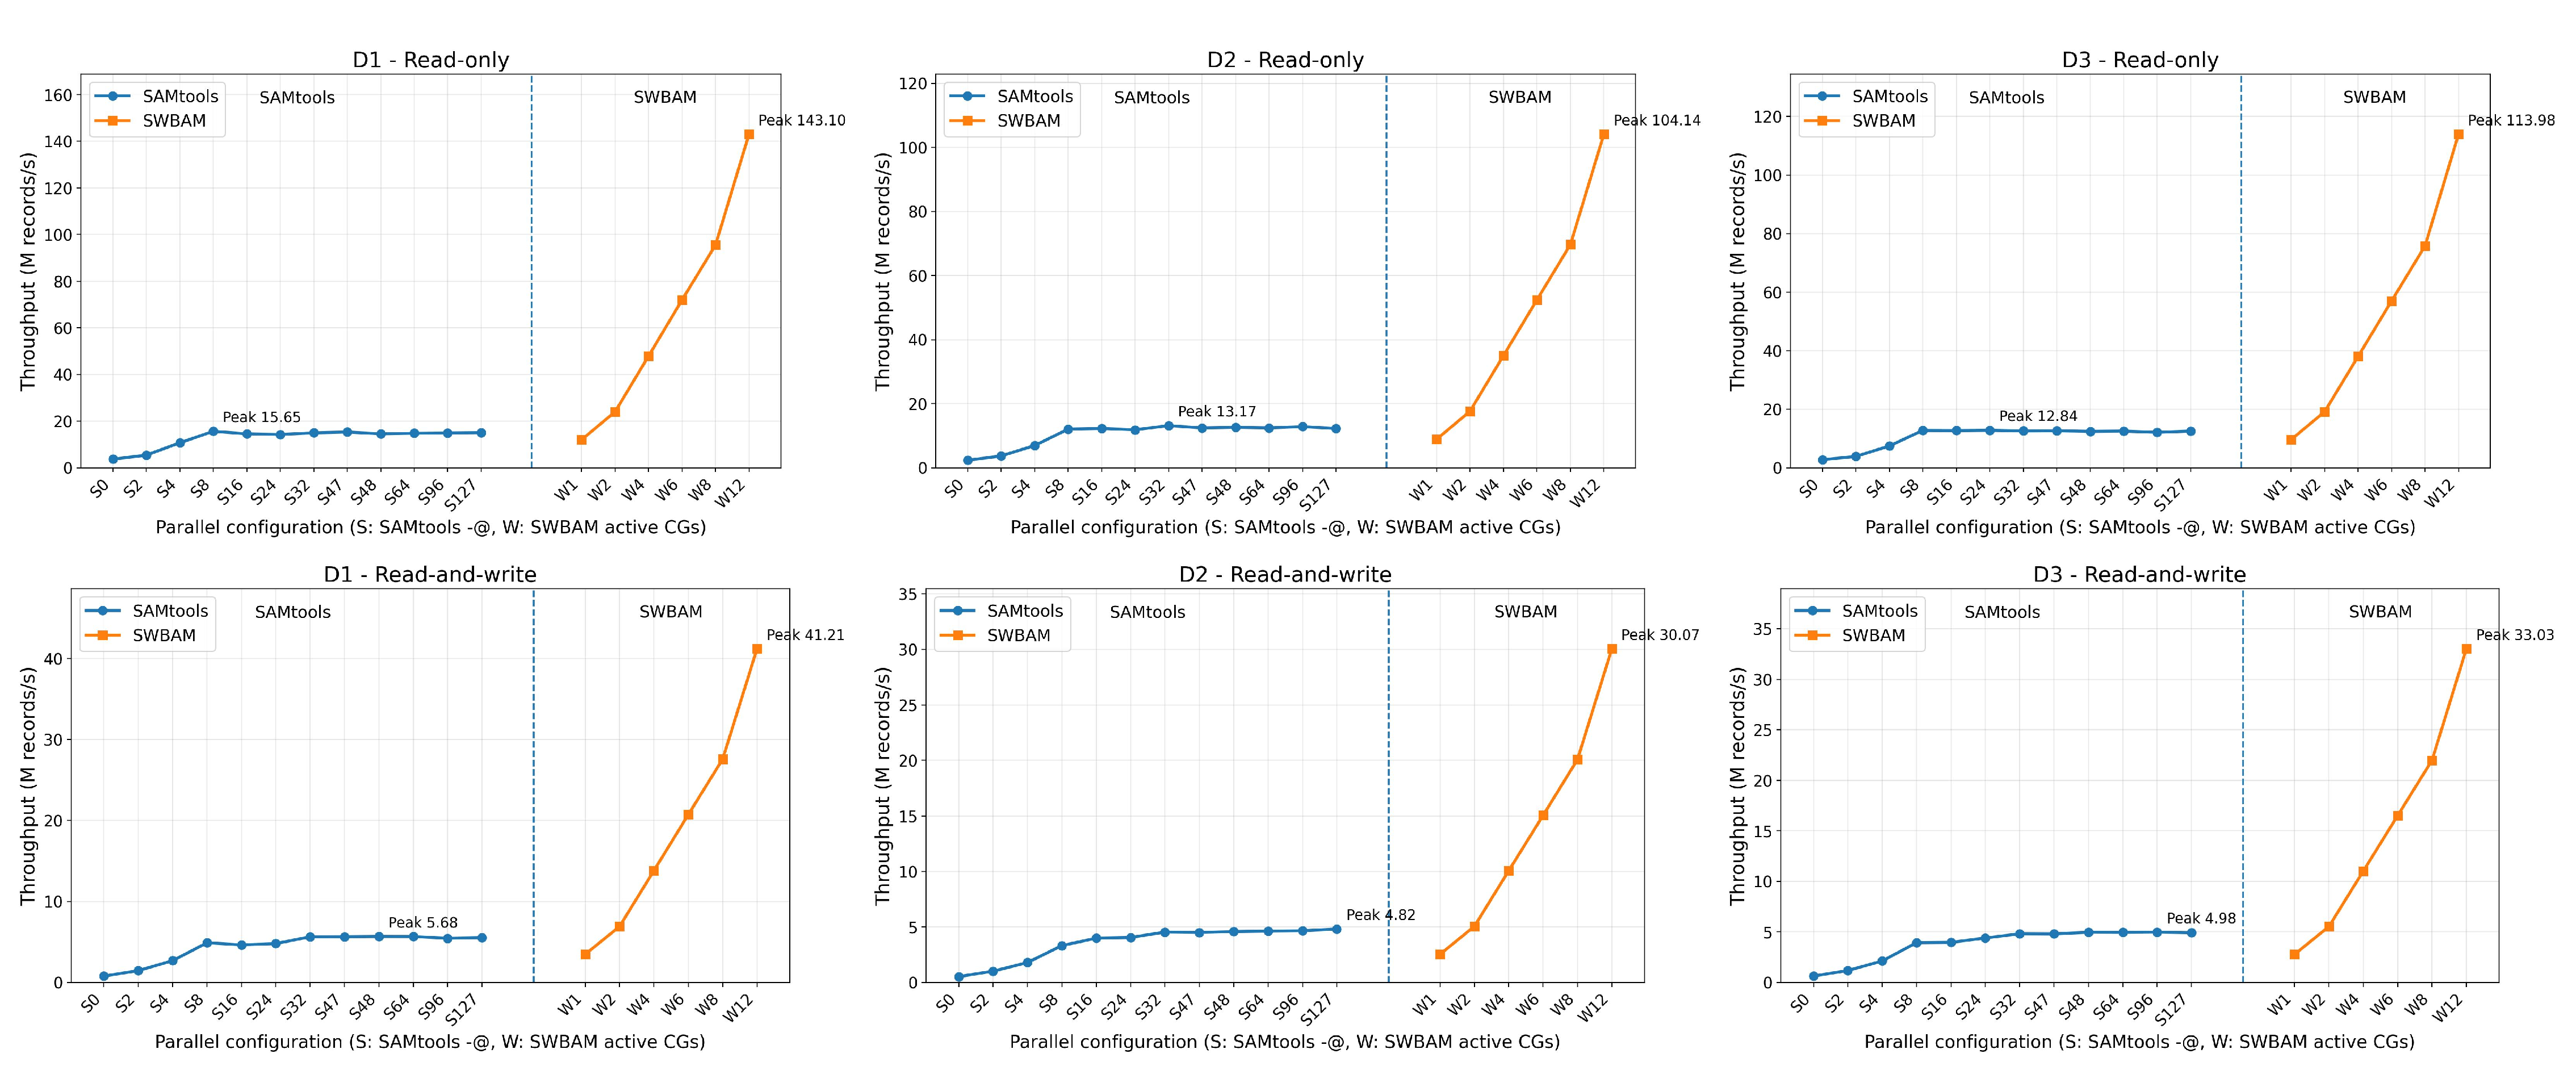
\includegraphics[width=\textwidth]{figs/swbam_library_io_combined.pdf}
\caption{Throughput and scalability of BAM read-only and read-and-write processing on D1--D3. The upper and lower rows show read-only and read-and-write results, respectively. Configurations labeled S denote SAMtools additional threads, while configurations labeled W denote SWBAM active core groups. Each point is calculated from the median execution time of three runs. SAMtools throughput uses wall time, while SWBAM throughput uses core pipeline time.}
\label{fig:lib_io_perf}
\end{figure*}

Fig.~\ref{fig:lib_io_perf} compares the two processing modes on D1--D3. The upper row presents read-only performance, and the lower row presents read-and-write performance. Within each panel, the configurations labeled S indicate the number of additional SAMtools threads specified by \texttt{-@}, while those labeled W indicate the number of active SWBAM core groups. Each active SWBAM core group uses one MPE and 64 CPEs, with one active group per allocated node. The two sections of the horizontal axis represent separate resource configurations rather than equivalent processor counts.

In read-only mode, SAMtools reaches a performance plateau after approximately eight additional threads, with limited improvements at higher thread counts. Its highest measured throughput is 15.65, 13.17, and 12.84 million records/s on D1, D2, and D3, respectively. These peaks occur at 8, 32, and 24 additional threads. In contrast, SWBAM maintains increasing throughput throughout the tested range of 1--12 active core groups. Its throughput increases from 12.04, 8.87, and 9.64 million records/s with one core group to 143.10, 104.14, and 113.98 million records/s with twelve core groups on D1--D3, respectively. Under the reported timing boundaries, the corresponding throughput ratios relative to the best measured SAMtools configurations are 9.14, 7.91, and 8.87.

Read-and-write processing exhibits lower throughput than read-only processing because it includes additional record serialization and BGZF compression. SAMtools reaches its highest measured throughput of 5.68, 4.82, and 4.98 million records/s on D1--D3 at 48, 127, and 96 additional threads, respectively. Compared with read-only processing, increasing the thread count remains beneficial over a wider range, although improvements become modest at higher thread counts. SWBAM continues to scale across the tested core-group configurations and reaches 41.21, 30.07, and 33.03 million records/s with twelve active core groups. The corresponding throughput ratios relative to the best measured SAMtools configurations are 7.25, 6.24, and 6.63.

SWBAM maintains near-linear strong scaling in both processing modes. Relative to its own single-core-group execution, read-only processing achieves speedups of 11.88, 11.74, and 11.83 with twelve active core groups on D1--D3, corresponding to parallel efficiencies of 99.0\%, 97.9\%, and 98.6\%. Read-and-write processing achieves approximately 11.88-fold speedups and 99.0\% parallel efficiency on all three datasets. These results show that the measured batch-processing pipelines scale effectively across the tested resources and dataset sizes. The contributions of individual MPE-CPE processing optimizations are examined in the following subsection.

\subsubsection{MPE-CPE processing performance}

\subsection{Performance of SWBAM Applications}
\subsubsection{Streaming BAM processing}
We evaluate flag statistics, mapping-quality filtering, and BAM/SAM format conversion as representative streaming applications. All SWBAM experiments use six active core groups, providing a total of six MPEs and 384 CPEs, with one active core group per node. For SAMtools, the thread settings are selected through preliminary tests on D1 and then applied to all three datasets. The selected numbers of additional threads are 8 for flagstat, 96 for filtering and BAM-to-SAM conversion, and 24 for SAM-to-BAM conversion. BAM output uses compression level 1 in both implementations.

%普通流式处理性能表
\begin{table}[!t]
\centering
\caption{Performance comparison of streaming BAM operations}
\label{tab:streaming_perf}
\setlength{\tabcolsep}{3pt}
\begin{tabular*}{\columnwidth}{@{\extracolsep{\fill}}lrrrrr@{}}
\toprule
& \multicolumn{2}{c}{Runtime (s)} & & \multicolumn{2}{c}{Parallel configuration} \\
\cmidrule(lr){2-3} \cmidrule(lr){5-6}
Application & SAMtools & SWBAM & Speedup & Threads & CGs \\
\midrule
\multicolumn{6}{c}{Dataset D1} \\
\midrule
Flag statistics & 12.24 & \textbf{3.61}  & 3.39 & 8  & 6 \\
MAPQ $\geq 30$  & 31.27 & \textbf{9.51}  & 3.29 & 96 & 6 \\
BAM-to-SAM      & 77.17 & \textbf{13.92} & 5.55 & 96 & 6 \\
SAM-to-BAM      & 38.01 & \textbf{11.96} & 3.18 & 24 & 6 \\
\midrule
\multicolumn{6}{c}{Dataset D2} \\
\midrule
Flag statistics & 28.37  & \textbf{9.21}  & 3.08 & 8  & 6 \\
MAPQ $\geq 30$  & 71.65  & \textbf{25.04} & 2.86 & 96 & 6 \\
BAM-to-SAM      & 211.11 & \textbf{35.24} & 5.99 & 96 & 6 \\
SAM-to-BAM      & 127.89 & \textbf{29.55} & 4.33 & 24 & 6 \\
\midrule
\multicolumn{6}{c}{Dataset D3} \\
\midrule
Flag statistics & 91.69  & \textbf{28.57} & 3.21 & 8  & 6 \\
MAPQ $\geq 30$  & 225.92 & \textbf{75.56} & 2.99 & 96 & 6 \\
BAM-to-SAM      & 659.73 & --             & --   & 96 & -- \\
SAM-to-BAM      & 418.31 & --             & --   & 24 & -- \\
\bottomrule
\end{tabular*}
\par\smallskip
\begin{minipage}{\columnwidth}
\footnotesize
Runtimes are medians of three runs. Speedup is calculated as the SAMtools runtime divided by the SWBAM runtime. Threads denotes the number of additional SAMtools threads, and CGs denotes the number of active SWBAM core groups. BAM output uses compression level 1. ``--'' indicates that the corresponding SWBAM experiment was not performed under the selected configuration.
\end{minipage}
\end{table}

Table~\ref{tab:streaming_perf} summarizes the speedups over SAMtools, calculated as the ratio of the median SAMtools time to the median SWBAM time across three runs. The reported ratios compare SAMtools wall time with SWBAM application processing time under the simulated-I/O configuration. The latter excludes physical input preparation and final file output.

For flag statistics, SWBAM achieves speedups of 3.39, 3.08, and 3.21 on D1, D2, and D3, respectively. This operation uses the BAM read pipeline to perform decompression, parsing, and record-level counting, followed by aggregation of the local results. For filtering with mapping quality $\geq 30$, the corresponding speedups are 3.29, 2.86, and 2.99. Unlike flag statistics, filtering additionally serializes and compresses the retained records through the BAM write pipeline. These results extend the library-level evaluation to statistical processing and selective BAM output.

Format conversion also benefits from the processing components provided by SWBAM. BAM-to-SAM conversion achieves speedups of 5.55 and 5.99 on D1 and D2, respectively, giving the largest ratios among the completed streaming comparisons. SAM-to-BAM conversion achieves speedups of 3.18 and 4.33 on the same datasets. The former connects the BAM read and SAM write pipelines, while the latter connects the SAM read and BAM write pipelines. D3 format conversion is not evaluated under the selected six-core-group memory configuration because of its high memory requirements.

Overall, the completed streaming comparisons show speedups ranging from 2.86 to 5.99 under the reported timing scopes. The results cover both read-only statistical processing and operations that generate BAM or SAM output. A direct speedup comparison between SWBAM \texttt{stats --basic} and SAMtools \texttt{stats} is excluded because the two commands compute different sets of statistics.

\subsubsection{Distributed BAM processing}

\subsection{Deduplication Workflow Performance}

\section{Conclusions}


\section*{Acknowledgments}


\bibliographystyle{unsrt}
\bibliography{ref}


%\newpage

% \section{Biography Section}
 
% \vspace{-4em}

% \begin{IEEEbiography}[{\includegraphics[width=1in,height=1.25in,clip,keepaspectratio]{figs/Lifeng Yan.png}}]{Lifeng Yan}
% received his bachelor’s degree from Shandong University in 2021. He is currently pursuing his Ph.D. at the School of Software, Shandong University, in Jinan. His primary research focus is on high-performance computing and bioinformatics, aiming to integrate cutting-edge software and hardware technologies with bioinformatics algorithms for faster large-scale data processing and analysis. 
% %He has won several first prizes in high-performance computing competitions, including ASC Student Supercomputer Challenge, PAC, and CPC Parallel Application Challenge.
% \end{IEEEbiography}
% \vspace{-2.4em}

% \begin{IEEEbiography}
% [{\includegraphics[width=1in,height=1.25in,clip,keepaspectratio]{figs/Zhan Zhao.png}}]{Zhan Zhao}
% received his bachelor’s and master’s degrees from the School of Software at Shandong University in 2021 and 2024, respectively. His research focuses on high-performance computing and bioinformatics, with achievements including first place in the National Parallel Application Challenge.
% \end{IEEEbiography}
% \vspace{-2.4em}

% \begin{IEEEbiography}
% [{\includegraphics[width=1in,height=1.25in,clip,keepaspectratio]{figs/Zekun Yin.png}}]{Zekun Yin}
% is an associate research professor at the School of Software, Shandong University. He received his bachelor’s and Ph.D. degrees from Shandong University in 2014 and 2020, respectively. His major research interests are high-performance computing and its application in life science and geoscience.
% %He is an expert in the design, implementation, and deployment of parallel bioinformatics algorithms, applications, and libraries on multi- and many-core HPC platforms. 
% He won the ACM Gordon Bell Prize in 2017 for his research work on the Tangshan earthquake simulation on the Sunway TaihuLight supercomputer.
% \end{IEEEbiography}
% \vspace{-2.4em}

% \begin{IEEEbiography}
% [{\includegraphics[width=1in,height=1.25in,clip,keepaspectratio]{figs/Tong Zhang.png}}]{Tong Zhang}
% received his bachelor’s and master’s degrees from Shandong University in 2020 and 2023, respectively. He is currently pursuing his Ph.D. at the School of Software, Shandong University, in Jinan. His primary research interests are high-performance computing and its applications in life sciences.
% \end{IEEEbiography}
% \vspace{-2.4em}

% \begin{IEEEbiography}
% [{\includegraphics[width=1in,height=1.25in,clip,keepaspectratio]{figs/Yang Yang.png}}]{Yang Yang}
% received her bachelor's degree from Shandong University in 2023. She is studying for a master's degree at the School of Software, Shandong University. Her main areas of study and research are high-performance computing and its applications in bioinformatics.
% \end{IEEEbiography}
% \vspace{-2.4em}


% \begin{IEEEbiography}
% [{\includegraphics[width=1in,height=1.25in,clip,keepaspectratio]{figs/Fangjin Zhu.png}}]{Fangjin Zhu}
% received his Ph.D. in Engineering and is currently a lecturer at Shandong University. His research interests encompass intelligent router technologies, swarm intelligence-based routing protocol design, virtual network technologies, computer network multicast algorithms, swarm intelligence optimization algorithms, and reinforcement learning algorithms. He has contributed to national and provincial research projects and has published over 20 papers in SCI/EI journals and conferences, including Computer Communications and IPCCC.
% \end{IEEEbiography}
% \vspace{-2.4em}

% \begin{IEEEbiography}
% [{\includegraphics[width=1in,height=1.25in,clip,keepaspectratio]{figs/Xiaohui Duan.png}}]{Xiaohui Duan}
% received a Ph.D. degree in computer science from Shandong University. He is currently a research professor at the School of Software, Shandong University. His research interests include HPC in molecular dynamics, earth system applications, and other problems with Sunway supercomputers.
% \end{IEEEbiography}
% \vspace{-2.4em}

% \begin{IEEEbiography}
% [{\includegraphics[width=1in,height=1.25in,clip,keepaspectratio]{figs/Bertil Schmidt.png}}]{Bertil Schmidt}
% is a tenured full professor and the Chair of Parallel and Distributed Architectures at Johannes Gutenberg University, Germany. His research group has developed various algorithms and tools for bioinformatics, focusing primarily on the analysis of large-scale sequence and short-read datasets, as well as data mining. Dr. Schmidt has received numerous accolades, including the CUDA Research Center Award, CUDA Academic Partnership Award, CUDA Professor Partnership Award, and Best Paper Awards at IEEE ASAP 2009 and IEEE ASAP 2015.
% \end{IEEEbiography}
% \vspace{-2.4em}


% \begin{IEEEbiography}
% [{\includegraphics[width=1in,height=1.25in,clip,keepaspectratio]{figs/Weiguo Liu.png}}]{Weiguo Liu}
% received the bachelor’s and master’s degrees from Xi’an JiaoTong University, China, and the Ph.D. degree from Nanyang Technological University, Singapore. He is currently a full professor and director with the High-performance Computing Lab, Shandong University. His research interests include HPC and data mining. He was nominated as ‘‘Taishan Scholar’’ in Shandong province, and received numerous awards (e.g., ACM Gordon Bell Prize award in SC 2017, Fraunhofer IGD Best Paper award, and CCF HPC China Best Paper Award). 
% \end{IEEEbiography}
% \vspace{-2.4em}

% \vfill


\end{document}


